\documentclass[a4paper, 11pt, oneside]{report} 
\usepackage[utf8]{inputenc}
\usepackage[dutch]{babel}
\usepackage{amsmath}
\usepackage{amsfonts}
\usepackage{amssymb}
\usepackage{graphicx}
\usepackage{caption}
\usepackage[table,xcdraw]{xcolor}
\usepackage[toc,page]{appendix}
\usepackage{hyperref}
\usepackage{titlesec}
\usepackage{listings}
\usepackage{float}
\usepackage{tikz}
\usetikzlibrary{trees}
\usepackage{tikz-qtree}
\usepackage{graphicx}
\usepackage{fancyref}
\usepackage{wrapfig}
\usepackage{url}
\usepackage{pdflscape}
\usepackage{fancyvrb}
\usepackage{fancyhdr}
\graphicspath{ {Afbeeldingen/} }
\usepackage{subfig}
\usepackage{tabularx}
\usepackage{apacite}
\usepackage{longtable}
\usepackage{titlecaps}
%\usepackage[T1]{fontenc}
\usepackage{titlesec, blindtext, color}
\definecolor{gray75}{gray}{0.75}
\newcommand{\hsp}{\hspace{20pt}}
\usepackage{pdfpages}
\usepackage{afterpage}


\newcolumntype{L}[1]{>{\raggedright\arraybackslash}p{#1}}

\titleformat{\chapter}[hang]{\huge\bfseries}{\thechapter\hsp\textcolor{gray75}{|}\hsp}{0pt}{\Large\bfseries}

\def\figureautorefname{Figuur}
\def\sectionautorefname{Paragraaf}
\def\chapterautorefname{Hoofdstuk}
\def\tableautorefname{Tabel}
\DeclareRobustCommand{\VAN}[3]{#2} % set up for citation

\lstset { %
	language=C++,
	backgroundcolor=\color{black!3}, % set backgroundcolor
	basicstyle=\footnotesize,% basic font setting
}

%% Sets page size and margins 
\usepackage[a4paper,top=3cm,bottom=3cm,left=3cm,right=3cm,marginparwidth=1.75cm]{geometry}

\author{M.W.J. Berentsen}
\font\myfont=cmr12 at 40pt
\title{\myfont Drone meshnetwerk simulatie}
\usepackage{titling}

\newcommand{\subtitle}[8]{%
	\posttitle{%
		\par\end{center}
	\begin{center}\large#1\end{center}
	\vskip0.5em
	\begin{center}\large#2\end{center}
	\begin{center}\large#3\end{center}
	\begin{center}\large#4\end{center}
	\begin{center}\large#5\end{center}
	\begin{center}\large#6\end{center}
	\begin{center}\large#7\end{center}
	\begin{center}\large#8\end{center}
	\vskip0.5em}%
}

\subtitle{Software Design Document}{HAN Arnhem}{561399}{MWJ.Berentsen@student.han.nl}{Versie 1}{Alten Nederland B.V.}{Docent: J. Visch, MSc}{Assessor: ir. C.G.R. van Uffelen}

\setlength{\parindent}{0pt}
\setlength{\parskip}{5pt plus 2pt minus 1pt}



\hypersetup{colorlinks=true, urlcolor=red,citecolor=black,linkcolor=blue}  % Colours hyperlinks in blue, but this can be distracting if there are many links.
\setcounter{tocdepth}{1}



\begin{document}
\begin{figure}
	\begin{center}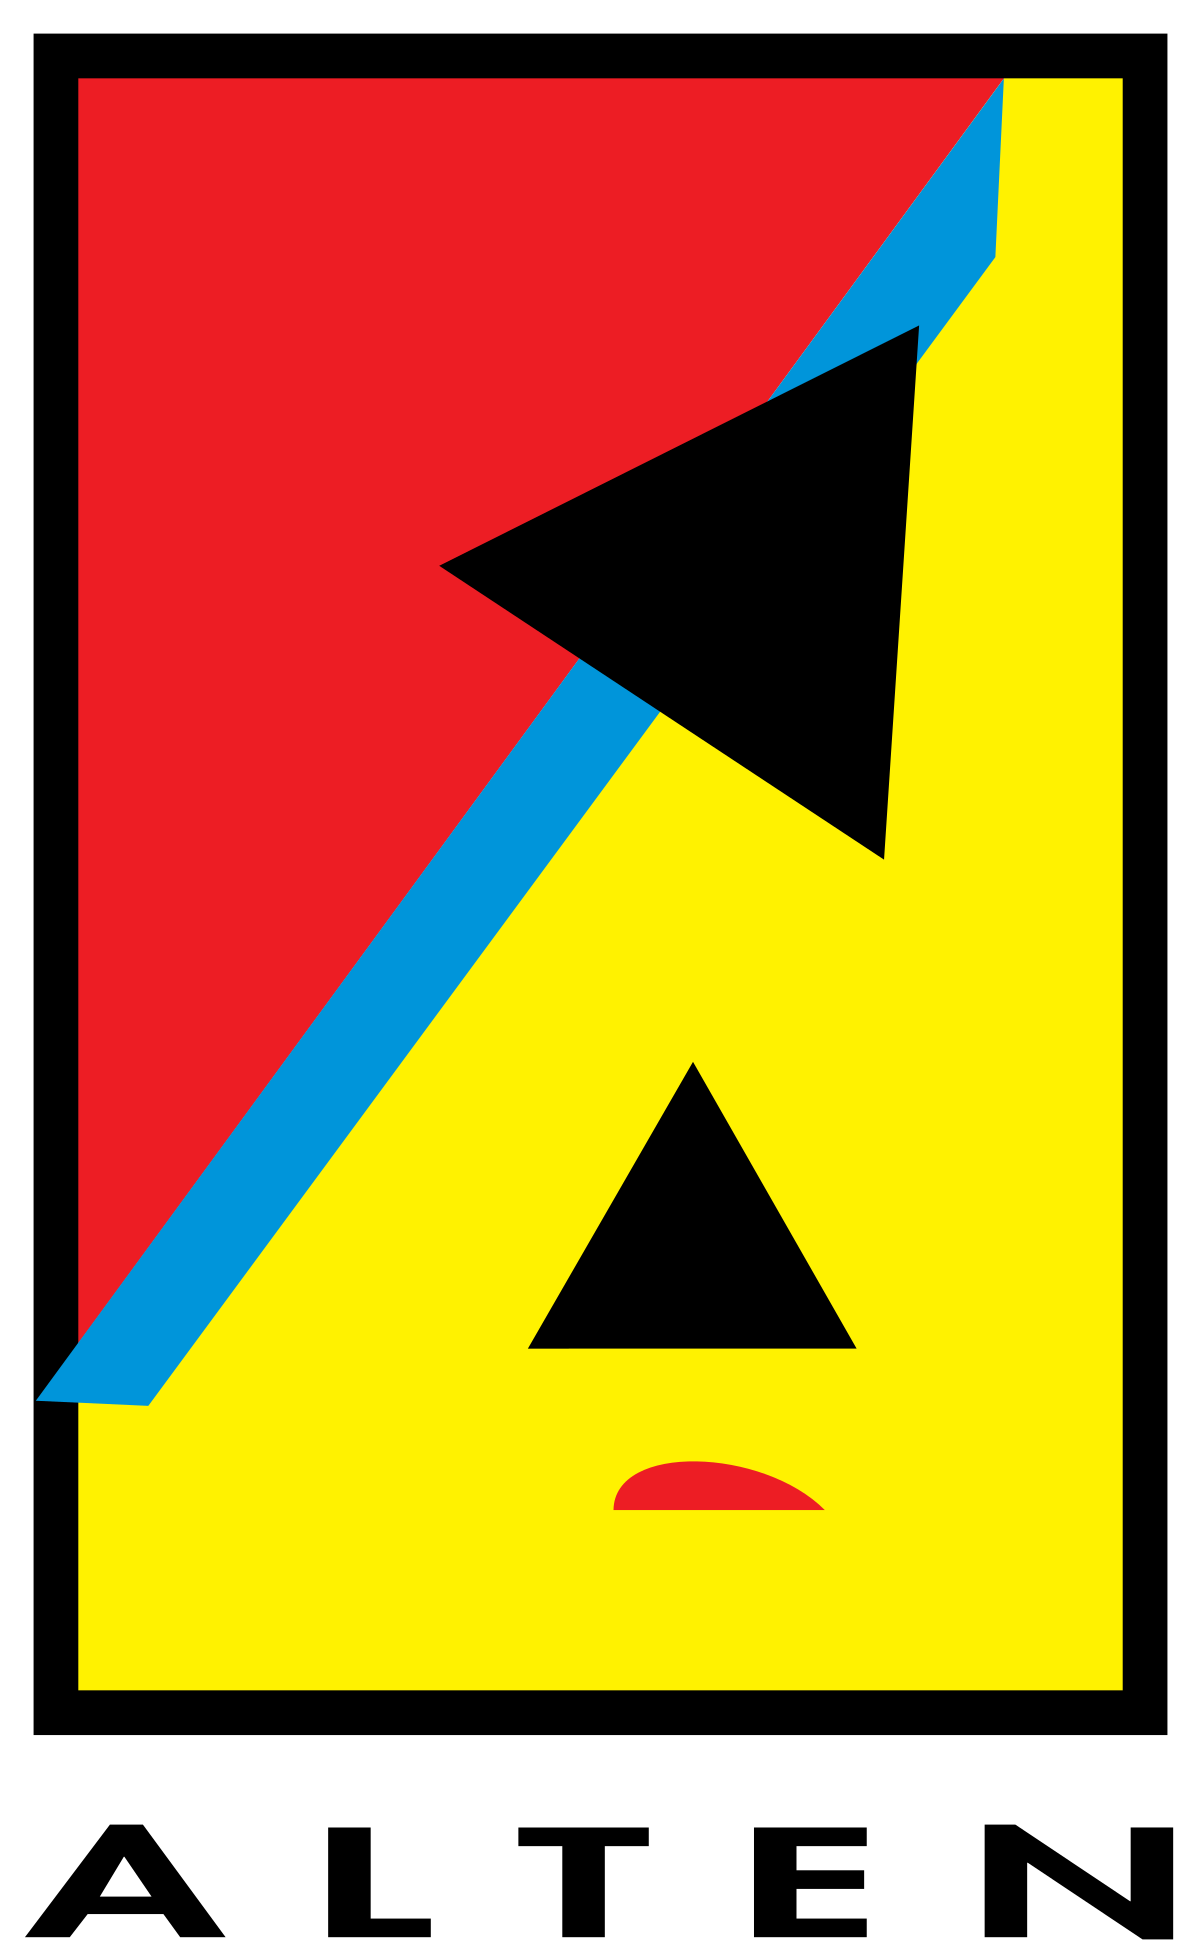
\includegraphics[scale=0.1]{alten}\end{center}
\end{figure}
\maketitle

%\section*{Voorwoord}
%\addcontentsline{toc}{section}{\protect\numberline{}Voorwoord}
%\pagebreak

%Geschikt voor minimaal 50 nodes; Kan slecht of geen signaal nabootsen

\tableofcontents
\clearpage


%\clearpage

%\section*{Samenvatting}
%\addcontentsline{toc}{section}{\protect\numberline{}Samenvatting}
%\pagebreak


\chapter{Inleiding}
\label{inleiding}
Het volgende verslag betreft de Software Requirements Specification voor de afstudeerstage van Maurice Berentsen (hierna: student).
Dit document volgt het document: \textit{"Software Design Description Template"} \cite{template:sdd}

Het beschrijft de hoe de uiteindelijke applicatie eruit zal zien en wat de functionaliteit hiervan zal zijn. Op de manier is het voor de student maar ook betrokken partijen duidelijk wat er gerealiseerd zal worden. Het verduidelijk de werking van de sub-componenten en de onderlinge relaties. 

\subsection{leeswijzer}
\label{inleiding:beschrijving:leeswijzer}
Eerst zal een korte beschrijving gegeven worden van het doel van dit document.Daarna wordt er door middel van een tabel een begrippenlijst toegelicht. In het tweede hoofdstuk is als eerste een component diagram te vinden waarin de functionaliteit van de verschillende componenten te vinden is en de manier waarop deze componenten met elkaar communiceren. Vervolgens is de algemene flow van het programma te zien, hierin wordt duidelijk welke stappen er onder water worden genomen als er een bepaalde actie wordt uitgevoerd. In hoofdstuk drie worden alle subsystemen duidelijk uitgewerkt en worden de ontwerpen van deze systemen uitgewerkt. 
\section{Begrippenlijst}
\label{inleiding:begrippenlijst}

% Please add the following required packages to your document preamble:
% \usepackage[table,xcdraw]{xcolor}
% If you use beamer only pass "xcolor=table" option, i.e. \documentclass[xcolor=table]{beamer}
\begin{table}[H]
\centering

\label{begrippen}
\begin{tabular}{|l|l|}
\hline
\rowcolor[HTML]{C0C0C0}
Term        & Omschrijving                                                         \\ \hline
term        & Omschrijving                                                      	\\ \hline

\end{tabular}
\caption{Begrippenlijst}
\end{table}

\chapter{Architectural Overview}
\label{architectural}
In het component diagram \autoref{fig:componentdiagram} op de volgende pagina is te zien dat bepaalde componenten voorzien zijn van een andere kleur. 
De groene kleur betekend dat het component voorzien is door gazebo.
De rode en blauw kleur zijn gegeneerd door ROS waarbij de rode een rosservice zijn en de blauwe een rostopic.
Op het hoogste niveau is het diagram te verdelen in vier groepen.

\textbf{Communication} is het component die de beslissingen neemt voor de communicatie.
Het heeft de intelligentie om het netwerk in kaart te brengen en te routeren.
Daarnaast is het in staat om een beslissing te nemen om een verzoek te sturen om de drone te verplaatsen.
Tenslotte bevat het meerdere berichten die gebruikt om het netwerk te kunnen onderhouden en op te bouwen.    

\textbf{Drone} is op dit moment een leeg component waar alleen een high level interface aanwezig is die de mogelijkheid biedt om de huidige locatie van een drone terug te geven of een nieuwe locatie als doel te geven aan de drone. 

\textbf{Gazebo} is de plek waar de virtualisatie van de drone plaats vindt.
Er kunnen virtuele router of gateway drones gemaakt worden die voorzien zijn van een virtuele arduino ingeladen met de juiste software en een virtuele drone motor.
Deze worden als model plug-in gekoppeld aan de drone in een gesimuleerde wereld waar Gazebo vervolgens physics op de drones kan uitvoeren. 

\textbf{ROS} is het component waar de simulatie van de communicatie plaats vindt.
Er is een virtuele NRF24 om te communiceren met andere nodes in het netwerk.
De aanwezige WirelessSignalSimulator zorgt dat dit realistisch gebeurd door alleen communicatie uit te voeren als dit volgens de voorwaarden mag.
Dit bepaald de simulator op basis van informatie die het krijgt van Gazebo en de NRF.
Tenslotte is er een DroneManager aanwezig die een interface aanbiedt via ros voor de ontwikkelaar om verbinding te maken met de gateways uit het netwerk.

\textbf{Arduino} is het component die zich onderscheid in twee rollen, een Arduino kan de rol van gateway hebben of de rol van router in de het meshnetwerk.

\textbf{NRF24} is het gebruikte component om draadloze communicatie mogelijk te maken. Het is voorzien van een driver in de vorm van een low level interface en bied zich aan via een high level interface voor communicatie.

Na het component diagram zal elke subcomponent kort toegelicht worden


\begin{landscape}
	\begin{figure}[p]%
		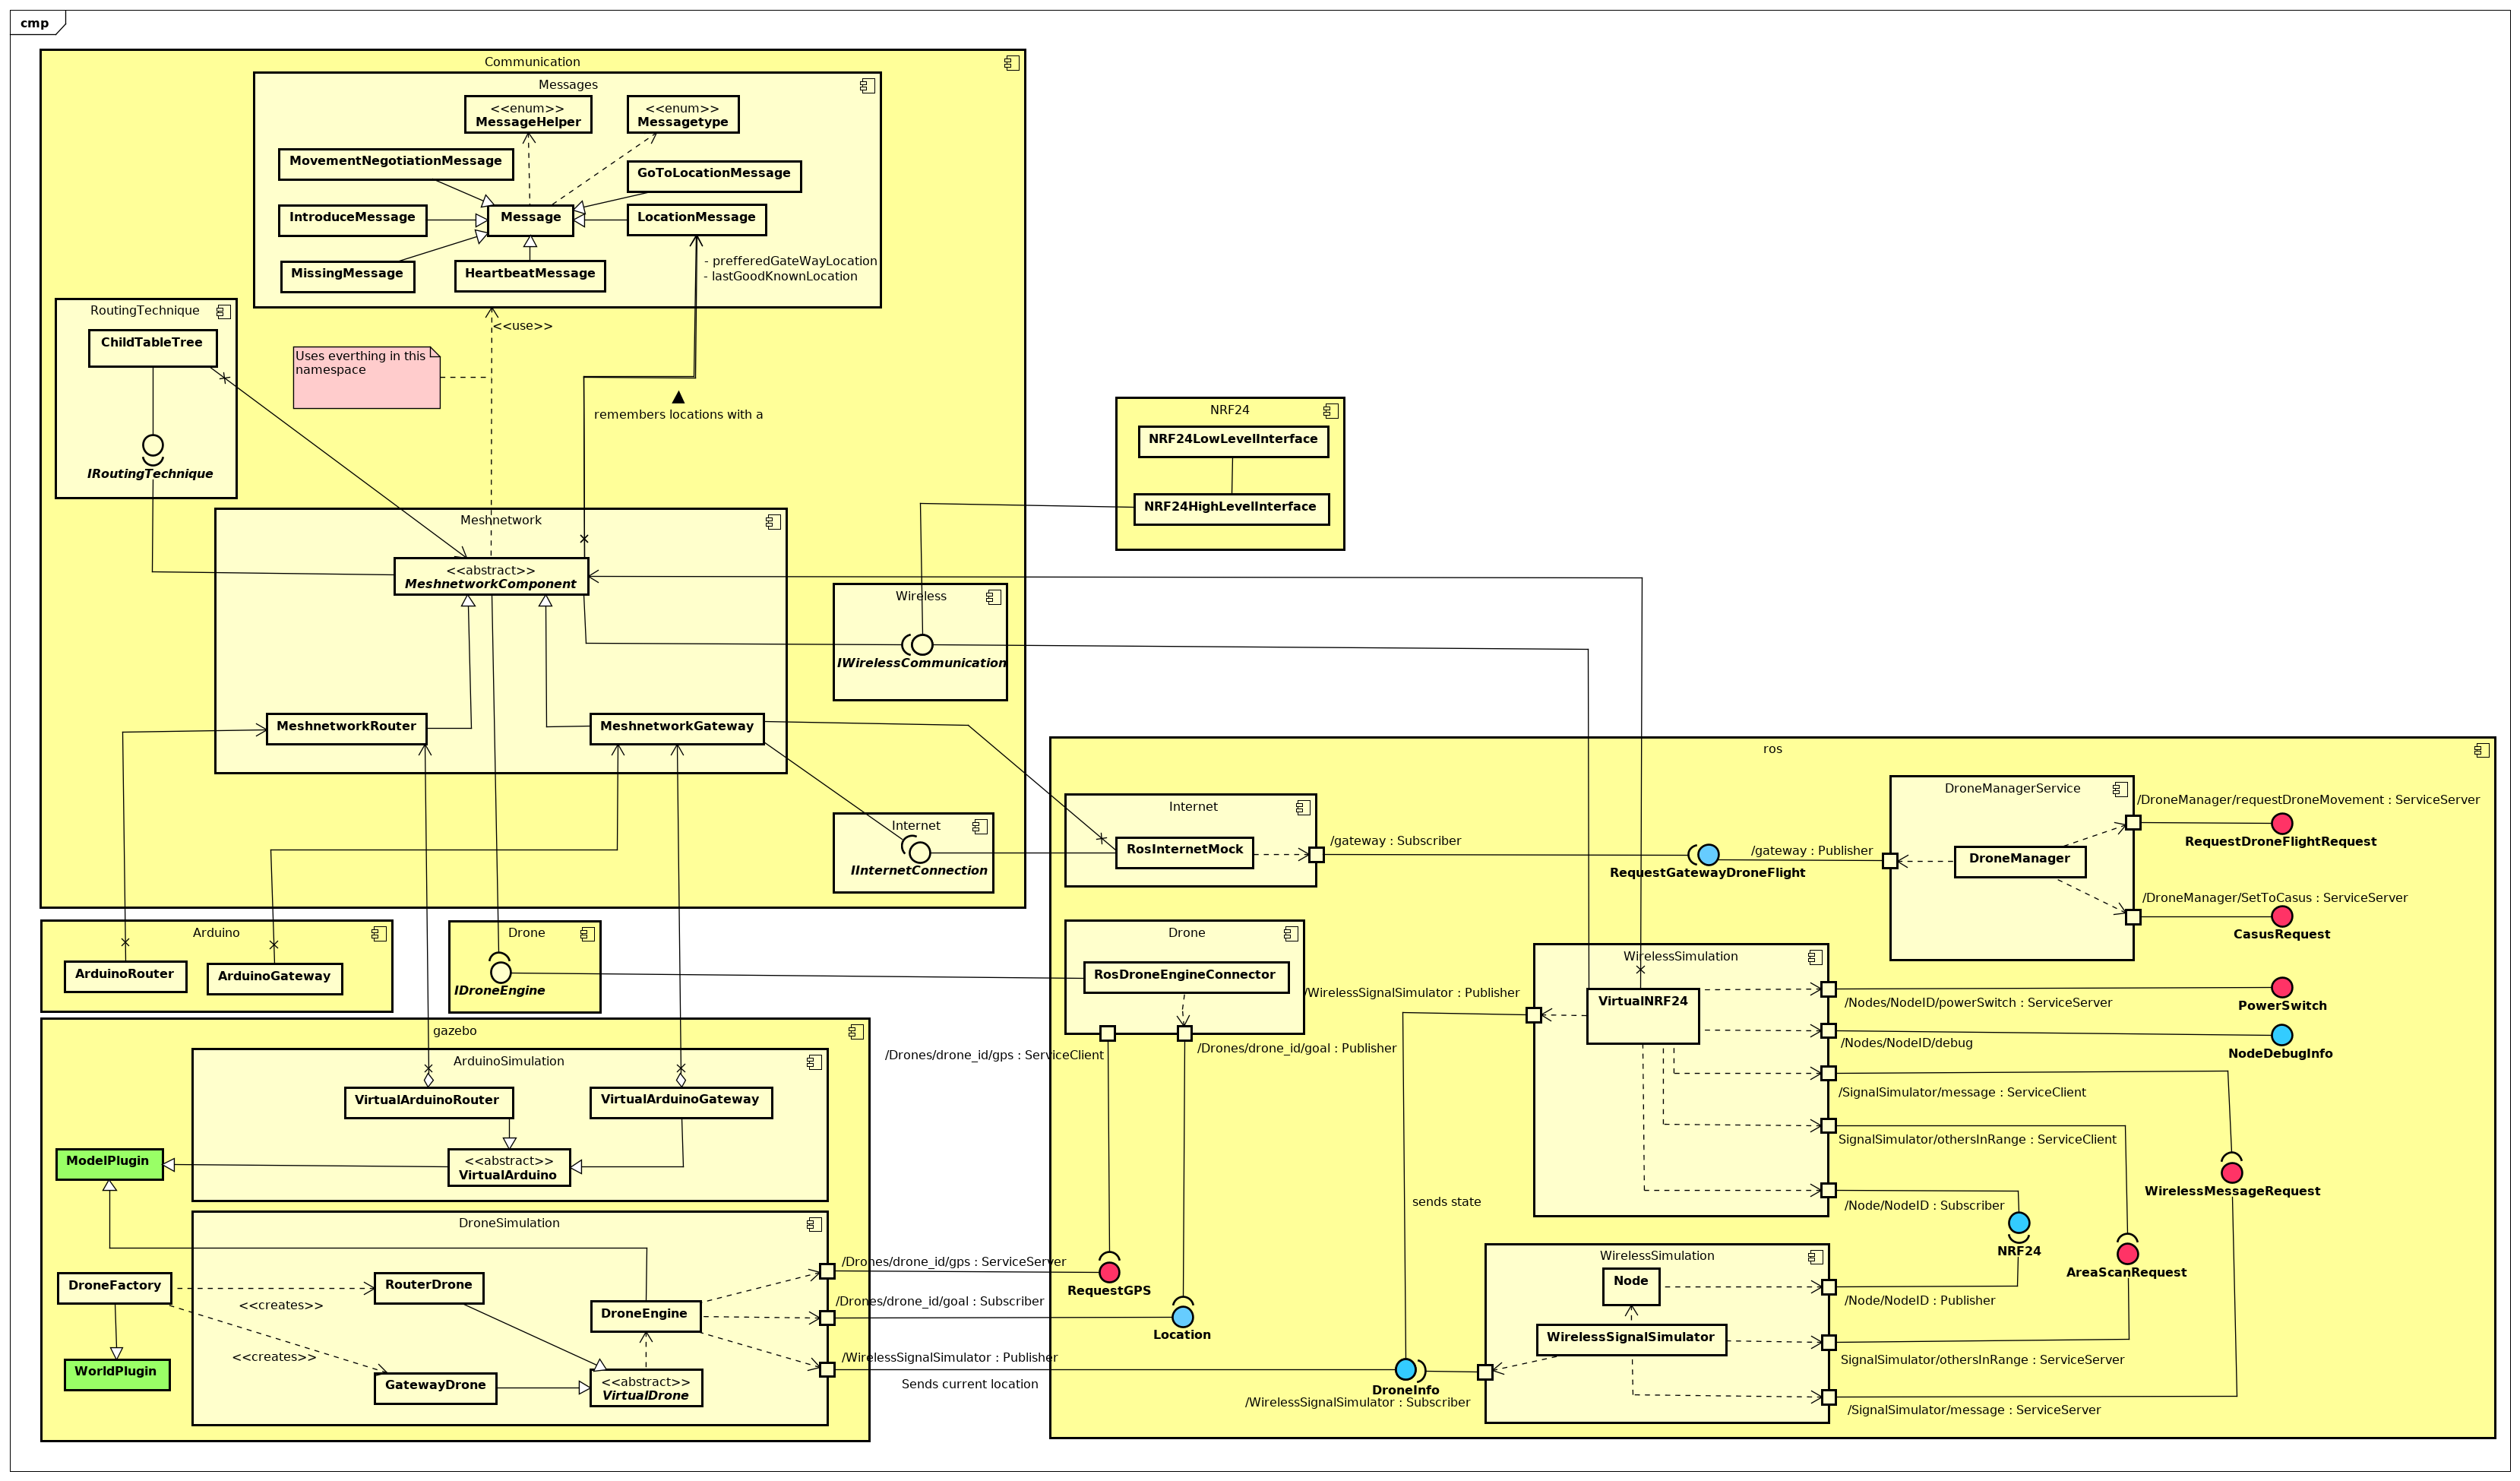
\includegraphics[width=\linewidth]{Afbeeldingen/ComponentDiagram.png}%
		\caption{Globale component diagram}
			\label{fig:componentdiagram}
	\end{figure}%
\clearpage
\end{landscape}
\clearpage



\section{Componenten}
\label{architectural:subcomponenten}

%NAMESPACE Communication
\subsection{Internet}
\label{architectural:subcomponenten:Internet}
Dit component bevat alleen een high level interface om verbinding te maken en te verbreken met het internet
\subsection{Meshnetwork}
\label{architectural:subcomponenten:Meshnetwork}
Dit component bevat de basis componenten voor het opbouwen van een meshnetwerk.
\subsection{MeshnetworkComponent}

\label{architectural:subcomponenten:MeshnetworkComponent}
Een MeshnetworkComponent is de basis van elk component in het mesh netwerk.
Het vereist routeringstechniek via de \nameref{architectural:interfaces:IRoutingTechnique}, een aansluiting naar een drone via \nameref{architectural:interfaces:IDroneEngine} en een vorm van draadloze communicatie via \nameref{architectural:interfaces:IWirelessCommunication}.
Hij maakt gebruikt van het component \nameref{architectural:subcomponenten:Messages} om te communiceren met andere MeshnetworkComponenten.
 
\subsection{MeshnetworkRouter}
\label{architectural:subcomponenten:MeshnetworkRouter}
Een meshnetwork router is een \nameref{architectural:subcomponenten:MeshnetworkComponent} die in staat is verbinding met andere nodes op te bouwen.
Zijn doel is om altijd verbinding te hebben met een \nameref{architectural:subcomponenten:MeshnetworkGateway}.
Als hij dit te lang niet heeft kan hij zich verplaatsen door aanspraak te maken op de DroneEngine.
Wanneer hij zich in een groep van andere Routers bevind zal hij eerst onderling onderhandelen wie er zich moet verplaatsen.

\subsection{MeshnetworkGateway}
\label{architectural:subcomponenten:MeshnetworkGateway}
De gateway is een \nameref{architectural:subcomponenten:MeshnetworkComponent} die in staat is een verbinding op te bouwen naar een punt buiten het meshnetwerk. In de huidige situatie kan dit via een internetverbinding die loopt via de interface \nameref{architectural:interfaces:IInternetConnection}. 

\subsection{Messages}
\label{architectural:subcomponenten:Messages}
Dit component betreft een verzameling van bericht samenstellingen die gebruikt worden voor de communicatie van het meshnetwerk.

\subsection{Message}
\label{architectural:subcomponenten:Message}
Een Message is de basis van elke bericht en bevat tenminste de volgende informatie:  Maker, zender, berichttype, ontvanger, geadresseerde. 
\subsection{GoToLocationMessage}
\label{architectural:subcomponenten:GoToLocationMessage}
Dit bericht bevat een locatie waar een drone zich naartoe moet verplaatsen.

\subsection{HeartbeatMessage}
\label{architectural:subcomponenten:HeartbeatMessage}
Dit bericht wordt gebruikt om de verbinding met anderen te onderhouden. Dit bericht maakt een hop per keer dat deze doorgestuurd wordt.

\subsection{IntroduceMessage}
\label{architectural:subcomponenten:IntroduceMessage}
Een introductie bericht wordt gebruikt door een node om schik voor te stellen aan alle andere nodes die dichtbij zijn. 

\subsection{LocationMessage}
\label{architectural:subcomponenten:LocationMessage}
Dit bericht wordt gebruikt om de huidige locatie van een node door te sturen naar een ander.

\subsection{MissingMessage}
\label{architectural:subcomponenten:MissingMessage}
Zodra een \nameref{architectural:subcomponenten:MeshnetworkComponent} de verbinding verliest met een ander gebruikt hij dit bericht om andere daarover te informeren.

\subsection{MovementNegotiationMessage}	
\label{architectural:subcomponenten:MovementNegotiationMessage}
Om onderling te onderhandelen tussen de nodes wie er actie moet ondernemen wordt dit bericht gebruikt.

\subsection{RoutingTechnique}
\label{architectural:subcomponenten:RoutingTechnique}
Dit component voorziet het meshnetwerk van een routing techniek wat dus inhoudt dat dit het component is die de communicatieroutes opbouwt naar andere punten in het netwerk.
  
\subsection{ChildTableTree}
\label{architectural:subcomponenten:ChildTableTree}
Deze techniek is een hybride meshnetwerk routing techniek waarbij een node de buren die deze heeft ziet als een kind.
Als een node een nieuw kind heeft vertelt hij dit aan zijn buren.
Omdat een node door zijn buren ook gezien wordt als kind registreren deze zijn nieuwe kind dus als kleinkind.
Hierdoor hoeft een node alleen maar te zoeken aan wie welk kind hij een bericht hoeft door te geven. 
De complexiteit van de routingtechniek neemt per stap in het netwerk af bij nodes met meerdere kinderen.
Als een drone zich verplaatst heeft wist deze het de opgebouwde geheugen van kinderen en kleinkinderen. 

\subsection{Wireless}
\label{architectural:subcomponenten:Wireless}
Dit component voorziet een \nameref{architectural:subcomponenten:MeshnetworkComponent} van een high level interface voor draadloze communicatie.
Als er een draadloos component wordt aangesloten moet deze hierop aangesloten worden. 

%NAMESPACE Drone
\subsection{Drone}
\label{architectural:subcomponenten:Drone}
Dit component representeert een drone. Omdat er op dit moment geen fysieke drone aanwezig is bezit deze component alleen een high level interface.
Deze interface is geschikt voor het ophalen van de huidige locatie en het ontvangen van een doellocatie

%NAMESPACE Arduino
\subsection{ArduinoRouter}
\label{architectural:subcomponenten:ArduinoRouter}
Dit component is een Arduino die voorzien is van een sketch om zich te gedragen als een router in het meshnetwerk
\subsection{ArduinoGateway}
\label{architectural:subcomponenten:ArduinoGateway}
Dit component is een Arduino die voorzien is van een sketch om zich te gedragen als een gateway in het meshnetwerk

%NAMESPACE GAZEBO
\subsection{ArduinoSimulation}
\label{architectural:subcomponenten:ArduinoSimulation}
In de dit component wordt een arduino gesimuleerd, deze simulatie is puur functioneel en betreft alleen een gelijk gedrag met betrekking tot de Arduino sketch. 
Het heeft geen effect op de clock snelheid deze is gelijk aan de computer waarop de software draait. 

\subsection{VirtualArduino}
\label{architectural:subcomponenten:VirtualArduino}
Dit abstracte component verplicht elke virtuele Arduino tot het aanmaken van een setup en loop functie zoals dit ook is in Arduino sketches.
Omdat deze Arduino altijd wordt toegevoegd aan een ander model erft dit component over van modelplugin.    
 
\subsection{VirtualArduinoRouter}
\label{architectural:subcomponenten:VirtualArduinoRouter}
Deze \nameref{architectural:subcomponenten:VirtualArduino} is voorzien van een sketch die de arduino zich laat gedragen als in router in het meshnetwerk. Dit component representeert het component \nameref{architectural:subcomponenten:ArduinoRouter} in gazebo.

\subsection{VirtualArduinoGateway}
\label{architectural:subcomponenten:VirtualArduinoGateway}
Deze \nameref{architectural:subcomponenten:VirtualArduino} is voorzien van een sketch die de arduino zich laat gedragen als in gateway in het meshnetwerk. Dit component representeert het component \nameref{architectural:subcomponenten:ArduinoGateway} in gazebo.


\subsection{DroneSimulation}
\label{architectural:subcomponenten:DroneSimulation}
Dit component is verantwoordelijk voor het simuleren van drones. 

\subsection{DroneEngine}
\label{architectural:subcomponenten:DroneEngine}
Elke \nameref{architectural:subcomponenten:VirtualDrone} is voorzien deze drone engine. 
Dit component maakt het mogelijk voor een drone om zich in een rechte lijn door lucht zich te verplaatsen waarbij het opstijgen en de landing verticaal wordt uitgevoerd.
Daarnaast biedt dit component via een rosservice het deel van de interface \nameref{architectural:interfaces:IDroneEngine} aan om de huidige locatie op te vragen.
Via een rostopic kan er een doel gestuurd gestuurd worden om het andere deel van de net genoemde interface te voorzien.
Tenslotte stuurt dit component bij elke verplaatsing de huidige locatie door naar de \nameref{architectural:subcomponenten:WirelessSignalSimulator}. 

\subsection{VirtualDrone}
\label{architectural:subcomponenten:VirtualDrone}
Een virtuele drone is een abstract component die alle variabelen bevat die nodig zijn om een drone in de wereld te injecteren. Deze variabelen betreffen een drone id, locatie en verwijzing naar de gazebo wereld. 

\subsection{GatewayDrone}
\label{architectural:subcomponenten:GatewayDrone}
Deze drone is een \nameref{architectural:subcomponenten:VirtualDrone} die in de sdf omschrijving wordt voorzien van een \nameref{architectural:subcomponenten:VirtualArduinoGateway} plugin. 
\subsection{RouterDrone}
\label{architectural:subcomponenten:RouterDrone}
Deze drone is een \nameref{architectural:subcomponenten:VirtualDrone} die in de sdf omschrijving wordt voorzien van een \nameref{architectural:subcomponenten:VirtualArduinoRouter} plugin. 

\subsection{DroneFactory}
\label{architectural:subcomponenten:DroneFactory}
Dit component is verantwoordelijk voor het produceren van drones. Het is een WorldPlugin die aan de hand van meegegeven parameters gateway en router drones aanmaakt.  

%NAMESPACE Ros
\subsection{RosDroneEngineConnector}
\label{architectural:subcomponenten:RosDroneEngineConnector}
Dit component is een adapter tussen de \nameref{architectural:subcomponenten:DroneEngine} en de interface \nameref{architectural:interfaces:IDroneEngine}. Die het mogelijk maakt om ros te gebruiken om aanspraak te maken op de virtuele drone.

\subsection{DroneManagerService}
\label{architectural:subcomponenten:DroneManagerService}
Dit component is de toegangspoort voor de ontwikkelaar tot de \nameref{architectural:subcomponenten:MeshnetworkGateway}.
Op dit moment is het component alleen geschikt om verplaatsingverzoeken te versturen via de gateway naar de Drones.
Hiervoor biedt het twee interfaces in de vorm van rosservices aan waarbij er een voor locaties is en de ander voor casussen. 

\subsection{DroneManager}
\label{architectural:subcomponenten:DroneManager}
Dit subcomponent realiseert de rosservices en publiceert verplaatsingverzoeken naar de gateways.  

\subsection{RosInternetMock}
\label{architectural:subcomponenten:RosInternetMock}
Deze internetmock laat de \nameref{architectural:subcomponenten:DroneManager} zich voordoen als internetpunt zodat er geen daadwerkelijke TCP/IP implementatie hoeft worden gemaakt 
\subsection{WirelessSimulation}
\label{architectural:subcomponenten:WirelessSimulation}
Het WirelessSimulation component is verantwoordelijk voor het simuleren van de NRF24 en het draadloze signaal hiervan. 
\subsection{WirelessSignalSimulator}
\label{architectural:subcomponenten:WirelessSignalSimulator}
Deze simulator bepaald of twee nodes met elkaar mogen communiceren. Het doet dit op basis van informatie die het continue ontvangt via het drone informatie topic. 
\subsection{Node}
\label{architectural:subcomponenten:Node}
Dit component wordt alleen gebruikt door de \nameref{architectural:subcomponenten:WirelessSignalSimulator} om te registreren welke Nodes bestaan, waar ze zijn en naar welk topic ze luisteren.
\subsection{VirtualNRF24}
\label{architectural:subcomponenten:VirtualNRF24}
Dit component is de virtuele versie van de NRF24, het is in staat om payloads te verwerken van 32 byte.
Deze kan de NRF24 naar een direct adres versturen of zenden naar alle NRF24 nodes binnen bereik.

\section{Interfaces}
\label{architectural:interfaces}
\subsection{IInternetConnection}
\label{architectural:interfaces:IInternetConnection}
Deze high level interface wordt gebruikt voor het leggen van een verbinding naar een extern punt buiten het netwerk. Omdat de gateway zich alleen hoeft te verbinden met een punt bestaat deze interface alleen uit een connect en een disconnect.
\subsection{IWirelessCommunication}
\label{architectural:interfaces:IWirelessCommunication}
In deze interface wordt de functionaliteit gesteld waar een draadloos communicatiemiddel aan moet voldoen. Het bevat functies om een antenne te starten en te stoppen. Het versturen van een bericht naar een specifiek punt of het zenden naar elke punt in de buurt. Er is een functie aanwezig om wanneer mogelijk debugging te gebruiken. Tenslotte moet een aansluitend component met deze interface moeten kunnen teruggeven of deze aan of uit staat.

\subsection{NRF24HighLevelInterface}
\label{architectural:interfaces:NRF24HighLevelInterface}

Deze high level interface is de aangeboden interface van de NRF24 en voldoet aan de interface \nameref{architectural:interfaces:IWirelessCommunication}. Het praat direct met de driver van de NRF24.  

\subsection{NRF24LowLevelInterface}
\label{architectural:interfaces:NRF24LowLevelInterface}
Deze low level interface is de driver van de NRF24


\subsection{IDroneEngine}
\label{architectural:interfaces:IDroneEngine}
Een drone engine interface representeert de aansluiting met een drone.
Hierin moet het mogelijk zijn om een doel coördinaat te sturen naar de drone om zich naartoe te verplaatsen. 
Daarnaast moet het mogelijk zijn voor een drone om de huidige positie terug te geven.
\subsection{IRoutingTechnique}
\label{architectural:interfaces:IRoutingTechnique}
Deze interface bevat functies voor het uitvoeren van een routeringstechniek.
Het heeft functies voor het starten en onderhouden van het netwerk.
Daarnaast zijn er functies hoe gereageerd moet worden op het vinden en verliezen van andere netwerkpunten.
Er zijn functies aanwezig om een adres op te halen waar naartoe gezonden moet worden om een punt te bereiken.
Ook kan er opgehaald worden welke punten zijn aangesloten, hoeveel punten dit zijn en hoeveel directe aansluitingen er zijn.
Tenslotte is er functie aanwezig die aangeroepen wordt zodra een drone zich verplaatst zodat hier adequaat op gereageerd kan worden.

\section{Ros topics en services}
\label{architectural:ros}
Zoals al eerder benoemd wordt er gebruik gemaakt van de transportlaag van ROS. Dit wordt gedaan in de vorm van Ros topics en services. Hieronder worden de messages en services kort toegelicht.
%ROS SERVICES
\subsection{RequestGatewayDroneFlight}
\label{architectural:ros:service:RequestGatewayDroneFlight}
Via deze aangeboden service is het mogelijk om een verzoek te sturen naar de gateway voor een verplaatsing. In het verzoek moet het nodeID en locatie zitten.


\subsection{CasusRequest}
\label{architectural:ros:service:CasusRequest}
Deze service maakt het mogelijk om een casus posities door te sturen naar de drones.

\subsection{PowerSwitch}
\label{architectural:ros:service:PowerSwitch}
Via deze simpele service kan een \nameref{architectural:subcomponenten:VirtualNRF24} aan of uit gezet worden.

\subsection{WirelessMessageRequest}
\label{architectural:ros:service:WirelessMessageRequest}
De \nameref{architectural:subcomponenten:VirtualNRF24} gebruikt deze service om een NRF24 bericht te versturen naar een andere NRF24. De response geeft aan of het zenden lukte.

\subsection{AreaScanRequest}
\label{architectural:ros:service:AreaScanRequest}
Deze service kan aangeroepen worden om de id's van alle nodes binnen het bereik van een node terug te krijgen. 
Dit is nodig om een algemene zending naar iedereen binnen bereik mogelijk te maken.

\subsection{RequestGPS}
\label{architectural:ros:service:RequestGPS}
Deze service wordt aangeboden door de \nameref{architectural:subcomponenten:DroneEngine} en biedt de mogelijkheid om de huidige locatie van een drone op te vragen. 

%ROS TOPICS
\subsection{RequestGatewayDroneFlight}
\label{architectural:ros:topic:RequestGatewayDroneFlight}
Dit topic wordt gebruikt om locatieverplaatsingverzoeken op te publiceren. 

\subsection{NodeDebugInfo}
\label{architectural:ros:topic:NodeDebugInfo}
Elke \nameref{architectural:subcomponenten:VirtualNRF24} maakt wanneer dit verzocht wordt een Debug topic aan. Hierop wordt informatie gepubliceerd wat van toegevoegde waarde is voor ontwikkelaars.

\subsection{NRF24}
\label{architectural:ros:topic:NRF24}
Een \nameref{architectural:subcomponenten:VirtualNRF24} luistert naar dit topic om zo berichten te kunnen ontvangen.

\subsection{Location}
\label{architectural:ros:topic:Location}
Het location topic representeert de verbinding die een \nameref{architectural:subcomponenten:MeshnetworkComponent} zou hebben met een drone op doelen op te versturen waar de Drone heen moet vliegen. 

\subsection{DroneInfo}
\label{architectural:ros:topic:DroneInfo}
Dit topic is essentieel voor de \nameref{architectural:subcomponenten:WirelessSignalSimulator}. De informatie die hierop gepubliceerd wordt omvat informatie over de locatie van een \nameref{architectural:subcomponenten:VirtualNRF24} of die aan staat en naar welk \nameref{architectural:ros:topic:NRF24} topic deze luistert.

\chapter{Detailed Design Description}
\label{DetailedDesign}

\section{Deployment Diagram}
\label{DetailedDesign:deployment}
In dit deployment diagram staan de executables (ROS nodes) die opgestart worden door de verschillende launch files, daarnaast zijn ook de twee ino files meegenomen die gebruikt worden bij de drones

\begin{figure}[H]
	\begin{center}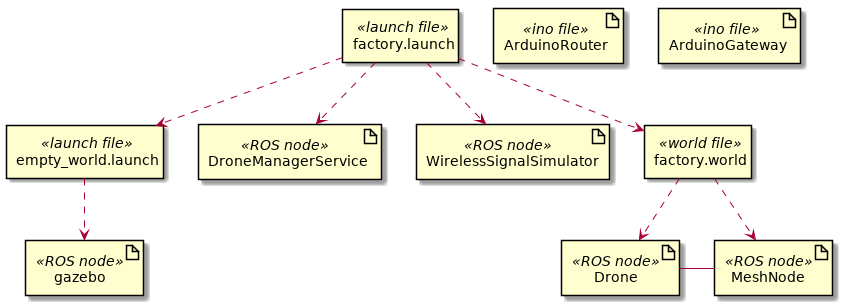
\includegraphics[width=\linewidth]{UML/out/DeploymentDiagram/DeploymentDiagram/DeploymentDiagram.png}\end{center}
	\caption{deployment diagram drone meshnetwerk}
	\label{fig:deploymentdiagram}
\end{figure}

\subsection{Ontwerpkeuzes met betrekking tot deployment}
\label{DetailedDesign:deployment:decisisions}

\subsubsection{Geen aangeboden mogelijkheid om drones los op te starten}
Er is voor gekozen om alleen via het factory.launch bestand de drones te kunnen starten. 
De factory.launch moet gebruikt worden omdat deze factory.world aanroept welke op zijn beurt de plugin start die de drones aanmaakt.  
In factory.world is het configureerbaar hoeveel gateway en router drones aangemaakt moeten worden.
Deze keuze is gemaakt omdat elke drone een uniek id moet hebben in de simulatie omdat elke motor zijn aansluiting publiceert aan de hand van dit id.

Om de gebruiker ervan te ontmoedigen is er daarom ook geen SDF bestand aanwezig waarmee normaal objecten in gazebo geladen worden. 

\section{Design Sub-Systeem Communicatie}
Het sub-systeem communicatie is verantwoordelijk voor de communicatie door het gebruik van mesh technologie.
Het subsysteem kan dit niet alleen en werkt daarom samen met andere subsystemen, welke zichtbaar zijn in het  \nameref{fig:componentdiagram}.
Het component communicatie bestaat ook weer uit kleinere componenten welke weergeven staan in het \nameref{fig:component:Communicatie}
  
\label{DetailedDesign:Communicatie}
\subsection{Component Diagram}
\label{DetailedDesign:CommunicatieComponentDiagram}
In de onderstaande afbeelding \ref{fig:component:Communicatie} staat het component diagram van de communicatie weergeven.
Het is een extractie uit het \nameref{fig:componentdiagram} 
\begin{figure}[H]
	\begin{center}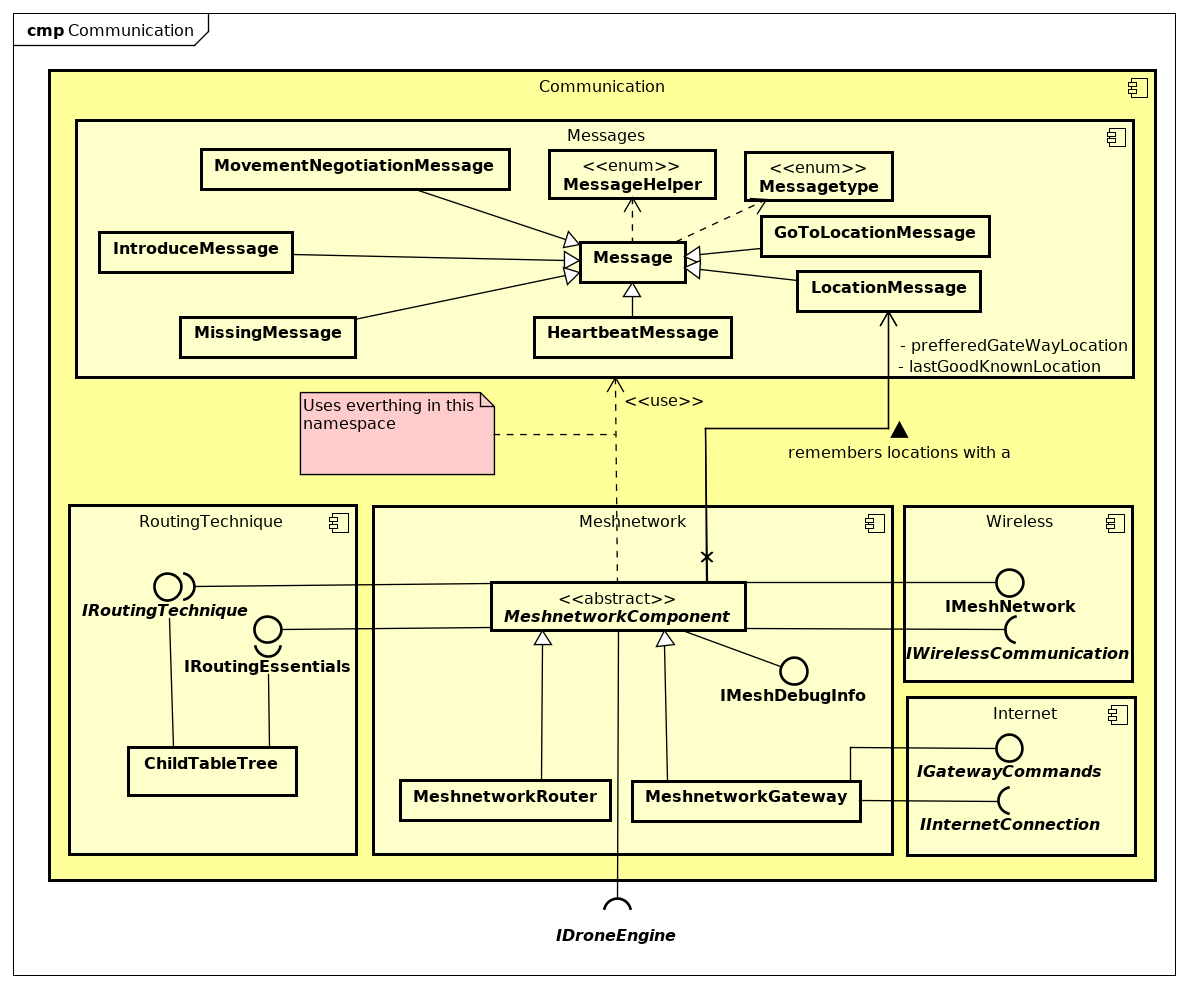
\includegraphics[width=\linewidth]{Afbeeldingen/CommunicationComponentDiagram.png}\end{center}
	\caption{Component diagram communicatie}
	\label{fig:component:Communicatie}
\end{figure}

\subsubsection{Interface beschrijving}
\label{DetailedDesign:CommunicatieComponentDiagram:interface}
Het communicatie component heeft geen aangeboden interfaces.
Wel wordt er intern een interface aangeboden door het subcomponent RoutingTechnique deze wordt hier behandeld. 

\paragraph{IRoutingTechnique}

De volgende functies worden aangeboden door de interface IRoutingTechnique. 

\begin{lstlisting}
uint8_t getDirectionToNode( const uint8_t node );

void startRouting( );

void maintainRouting( );

void NodeMovedLocation( );

uint8_t cantCommunicateWithNode(const uint8_t node);

uint8_t OtherCantCommunicateWithNode(const uint8_t other, const uint8_t node);

void canCommunicateWithNode(const uint8_t node);

void OtherCanCommunicateWithNode(const uint8_t other, const uint8_t node);

const uint16_t getTableSize( );

const uint16_t getAmountOfChildren( );

const std::set< uint8_t > getSetOfChildren( );

const bool empty( );
\end{lstlisting}
\subsection{getDirectionToNode}
Deze functie is de functie waar de aanvragende interface het meeste belang bij heeft.
Deze functie verwacht een id van de geadresseerde node als parameter.
De routing techniek zal vervolgens uitzoeken naar welke node een bericht doorgegeven moet worden om het bericht aan te laten komen bij de geadresseerde.
Dit adres wordt terug gegeven als een return waarde. 

\textbf{\textit{preconditie:}} Geadresseerde is bekend bij de routing techniek.

\textbf{\textit{postconditie:}} Routing techniek geeft terug welk adres het vervolg adres is voor het bericht.

\subsection{startRouting}
De functie start routing wordt aangeroepen zodra de routing techniek moet beginnen met het opbouwen van communicatie routes.

\textbf{\textit{preconditie:}} Het communicatie waarover de routering gebeurd is beschikbaar

\textbf{\textit{postconditie:}} De node zich aangemeld bij andere nodes en kan adressen opslaan.

\subsection{maintainRouting}
Deze functie wordt herhaaldelijk aangeroepen in de software.
Het roept de routing techniek aan om een onderhoud te plegen aan de opgebouwde routing informatie.
Zo zal vaak het geval zijn dat de routing techniek controleert of de aansluitende nodes nog bestaan.

\textbf{\textit{preconditie:}} De routing techniek is gestart met routeren en heeft een lijst van beschikbare nodes.

\textbf{\textit{postconditie:}} Er is onderhoud uitgevoerd aan de lijst van beschikbare nodes.

\subsection{NodeMovedLocation} 
Deze functie wordt aangeroepen zodra de drone zich verplaatst heeft. Het is aan routing techniek om hier adequaat op te reageren.
In de huidige implementatie worden alle routes als ongeldig gezien waardoor de tabel geleegd wordt. 

\textbf{\textit{preconditie:}} Er is geen preconditie.

\textbf{\textit{postconditie:}} De routeringstechniek heeft de tabel bij adequaat bijgewerkt.


\subsection{cantCommunicateWithNode} 
Deze functie wordt aangeroepen als er geen connectie gelegd kan worden met een node. Deze functie geeft terug op hoeveel routes de node had in het netwerk. 

\textbf{\textit{preconditie:}} De node is aanwezig in de route tabel.

\textbf{\textit{postconditie:}} De route wordt verwijderd of als niet beschikbaar beschouwd.


\subsection{OtherCantCommunicateWithNode}
Deze functie wordt aangeroepen als een andere node aangeeft dat hij geen connectie kan maken met een node. Deze functie geeft terug op hoeveel routes de niet bereikbare node voorkomt. 

\textbf{\textit{preconditie:}} De node is aanwezig in de route tabel.

\textbf{\textit{postconditie:}} De route wordt verwijderd of als niet beschikbaar beschouwd.

\subsection{canCommunicateWithNode}
Zodra een node bevestiging heeft dat deze verbinding kan maken wordt deze functie aangeroepen. Als parameter wordt het adres meegegeven.

\textbf{\textit{preconditie:}} Er is bevestiging dat een node een directe verbinding heeft met een andere node.

\textbf{\textit{postconditie:}} De verbonden node wordt toegevoegd als direct route punt.
 
\subsection{OtherCanCommunicateWithNode}
De functie wordt aangeroepen als een andere node doorstuurt dat hij bevestiging heeft dat hij verbinding heeft met een nieuwe node in het netwerk. Als parameter wordt het adres meegegeven van zowel de node die aangeeft dat hij een verbinding heeft gevonden als het adres die hij gevonden heeft.

\textbf{\textit{preconditie:}}  Er is bevestiging dat een node een verbinding heeft met een andere node.

\textbf{\textit{postconditie:}}  De gevonden node wordt toegevoegd als route punt in het netwerk.


\subsection{getTableSize}
Deze functie geeft terug hoeveel routes er zich bevinden in de opgebouwde routing tabel.

\textbf{\textit{preconditie:}} Geen pre conditie.

\textbf{\textit{postconditie:}} Alle routes zijn geteld en de functie geeft dit aantal terug

\subsection{getAmountOfChildren}
In deze functie wordt het aantal gevonden direct aansluitende nodes geteld en terug gegeven.  

\textbf{\textit{preconditie:}}  Geen preconditie

\textbf{\textit{postconditie:}} Het aantal direct aansluitende nodes is geteld en en dit aantal is terug gegeven.

\subsection{getSetOfChildren}
Hier wordt een set gemaakt met id's van direct aansluitende nodes 
\textbf{\textit{preconditie:}} Geen preconditie

\textbf{\textit{postconditie:}} Er is een set met de id's van alle nodes waar een directe verbinding mee gevonden is

\subsection{empty}
Deze functie geeft een bolean terug welke aangeeft of de tabel leeg is.
Dit is een aparte functie omdat het scheelt in complexiteit ten opzichte van het tellen van een tabel en die vergelijken met 0.
  
\textbf{\textit{preconditie:}} Geen preconditie

\textbf{\textit{postconditie:}} Er is een check gedaan of de lijst leeg is en dit wordt terug gegeven.

\subsection{Sequence Diagrams}
\label{DetailedDesign:Communicatie:sequence}
Hier worden aan de hand van sequence diagrammen communicatie wegen omschreven die zich binnen het component afspelen.

\subsubsection{Heartbeat van router naar gateway met directe verbinding}
\label{DetailedDesign:Communicatie:sequence:heartbeatrouter->gateway}
Om duidelijk te maken hoe een bericht van een node naar een gateway komt wordt het scenario van een heartbeat uitgewerkt in een direct verbinden.
Deze weg van communicatie wordt voor alle directe berichten het zelfde uitgevoerd.
Dat maakt het overbodig om voor elk type bericht een sequence diagram uit te werken
\begin{figure}[H]
	\begin{center}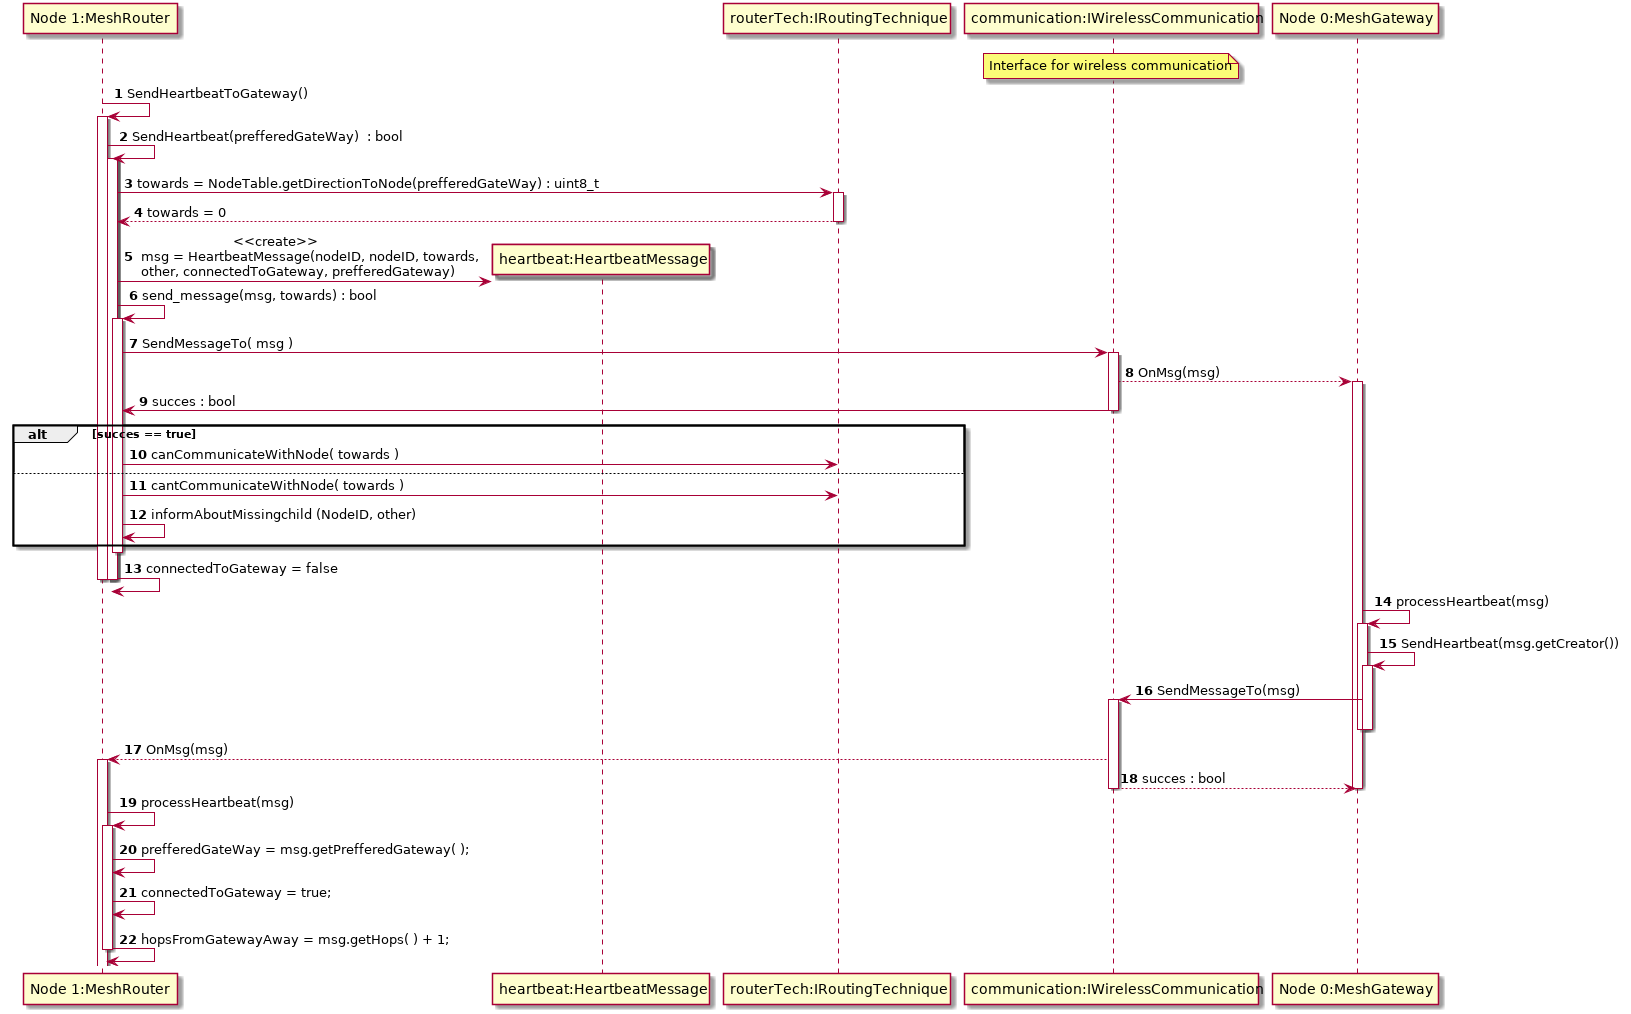
\includegraphics[width=.97\linewidth]{UML/out/Communication/Sequence/RouterDirectNaarGatewayHeartbeat/RouterDirectNaarGatewayHeartbeat.png}\end{center}
	\caption{Sequence diagram van een heartbeat bericht van een router naar een gateway met een directe onderlinge verbinding.}
	\label{fig:communication:sequence:sequence:heartbeatrouter->gateway}
\end{figure}
In diagram \ref{fig:communication:sequence:sequence:heartbeatrouter->gateway} is de flow zichtbaar van een router die een heartbeat bericht verstuurd naar een gateway en daar ook weer response op krijgt.
Op het moment dat een router het bericht om een heartbeat te versturen naar de gateway zal hij dit altijd doen naar de gateway waar hij een voorkeursverbinding (prefferedGateway) mee heeft.
Hij zal aan de aangesloten routeringstechniek vragen of er een route mogelijk is naar de router een aan wie hij zijn bericht dan moet afgegeven.
In het geval van deze sequence diagram heeft de router een directe verbinding met de gateway en is in stap 4 te zien dat het teruggegeven adres 0 is het adres van de gateway.

Vervolgens maakt de router een heartbeat bericht aan die het via de \nameref{architectural:interfaces:IWirelessCommunication} interface verstuurd naar de Gateway.
De router geeft door aan de routeringstechniek in stap 10 of 11 of het zenden wel of niet gelukt is op basis van de succes feedback uit stap 9.
Als het niet lukt geeft hij dit ook door aan zijn aangesloten punten in stap 12 %TODO referentie naar hoe die werkt
Als laatste voordat de router zijn functie verlaat zet hij in stap 13 de boolean die bijhoudt of verbinding is met de gateway (connectedToGateway) op false omdat hij verwacht dat er reactie komt van de gateway die het weer op true zet.

Bij stap 8 is het gelukt om het bericht te versturen naar de gateway die daar via zijn eigen \nameref{architectural:interfaces:IWirelessCommunication} interface het bericht ontvangt.
Er is voor gekozen om deze interface maar één keer weer te geven in de tabel om het overzichtelijk te houden.
De reactie van een gateway op een heartbeat is altijd dat er een heartbeat wordt teruggestuurd naar de zender. 
De functie SendHeartbeat(uint8\textunderscore t) in stap 15 werkt gelijk aan die van stap 2 en is daarom niet opnieuw uitgewerkt.

Stap 17 is het moment dat de router weer response heeft van de gateway.
Hij stelt op basis van de inhoud van het bericht het ID van de gateway in als prefferedGateway, zet de boolean connectedToGateway weer op true en registreert hoeveel hops het bericht nodig had om aan te komen.

\subsubsection{Heartbeat van gateway naar een router via een andere router}
\label{DetailedDesign:Communicatie:sequence:heartbeatgateway->router->router}

\begin{figure}[H]
	\begin{center}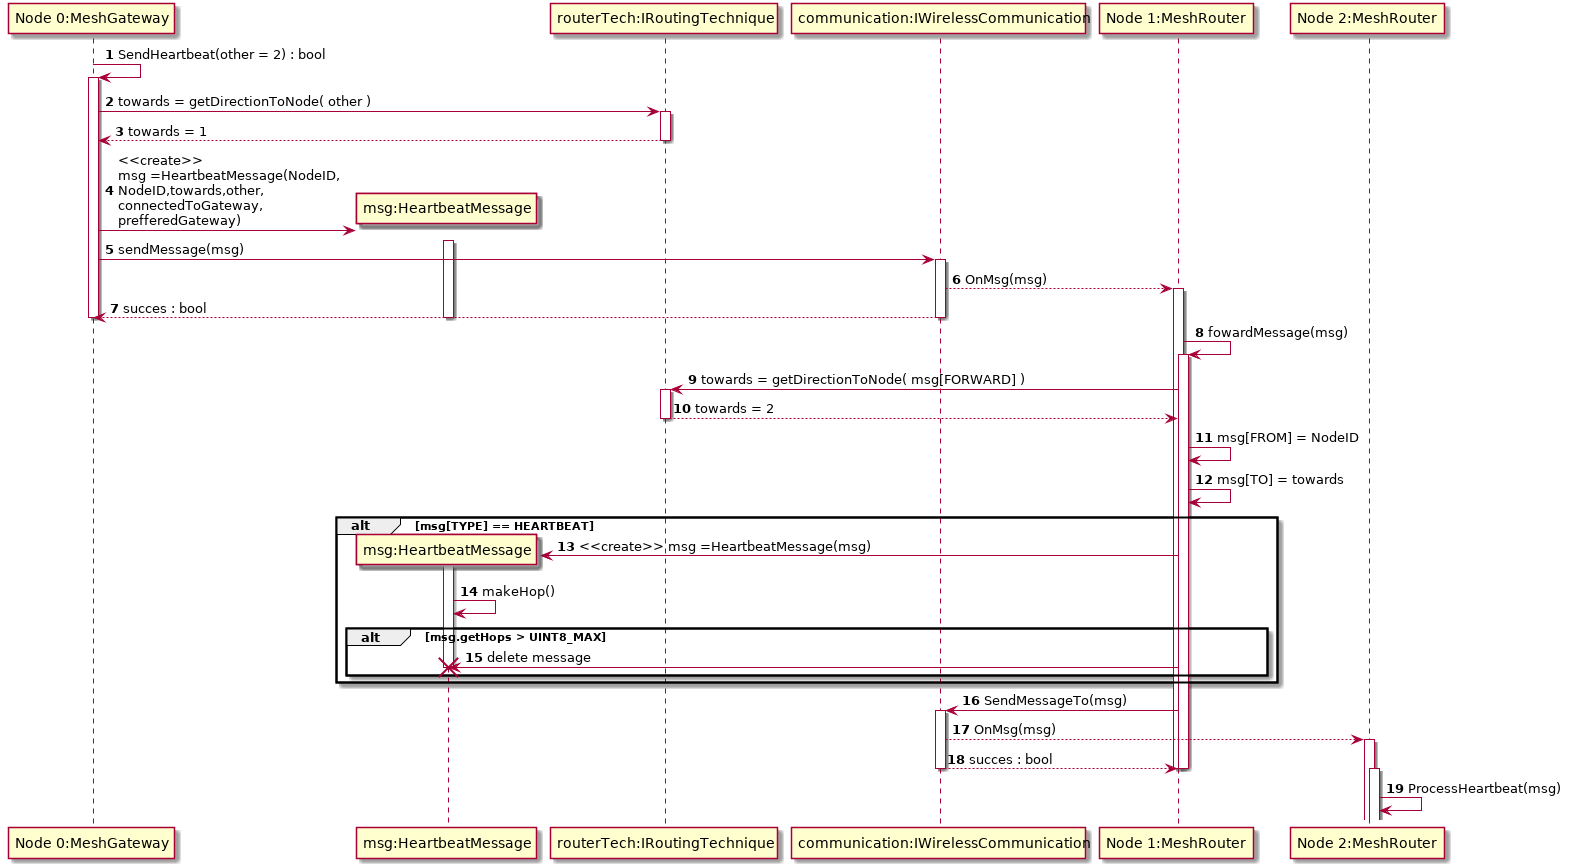
\includegraphics[width=\linewidth]{UML/out/Communication/Sequence/ForwardHeartbeat/ForwardHeartbeat.png}\end{center}
	\caption{Sequence diagram van een heartbeat bericht van een gateway naar een router via een andere router.}
	\label{fig:communication:sequence:sequence:heartbeatgateway->router->router}
\end{figure}
Diagram \ref{fig:communication:sequence:sequence:heartbeatgateway->router->router} laat zien hoe een heartbeat verstuurd wordt vanaf een gateway naar een router via een andere router.
Er is gekozen om de flow van een heartbeat bericht te laten zien omdat deze bij een forward ook een hop extra krijgt en daarmee het meest complex is.
Elke node heeft een eigen instantie van een routeringstechniek en draadloze communicatie, in deze diagram is gekozen om dezelfde te gebruiken om de leesbaarheid goed te houden.

Bij stap 3 is zichtbaar dat de routeringstechniek bij aanvraag voor een route naar node 2 een adres teruggegeven wordt van node 1 omdat via deze weg het bericht doorgegeven moet worden.
Vanaf stap 8 is zichtbaar wat er gebeurd als een bericht doorgestuurd moet worden.
Bij stap 9 wordt er eerst gekeken of er een route is naar de geadresseerde en aan wie het bericht dan doorgegeven moet worden.
Node 1 heeft een directe verbinding met node 2 dit wordt dan ook als adres doorgegeven in stap 10.
Vervolgens past de meshrouter het bericht aan dat zodat de zender en ontvanger weer juist staan. 
De waardes waar in staat wie de geadresseerde en maker van het bericht zijn blijven onaangepast.
Als het bericht van het type heartbeat is wordt deze apart genomen om er in stap 14 een hop bij op te tellen.
Als een heartbeat bericht meer hops heeft gemaakt dan dat er in de waarde van hop past wordt het bericht verwijderd en de flow gestopt.

In stap 16 wordt het bericht doorgestuurd naar de geadresseerde.
Als het bericht een heartbeat was wordt deze doorgestuurd anders wordt het aangepaste bericht verstuurt.

\subsubsection{Heartbeat van een router naar een andere router}
\label{DetailedDesign:Communicatie:sequence:heartbeatrouter->router}
\begin{figure}[H]
	\begin{center}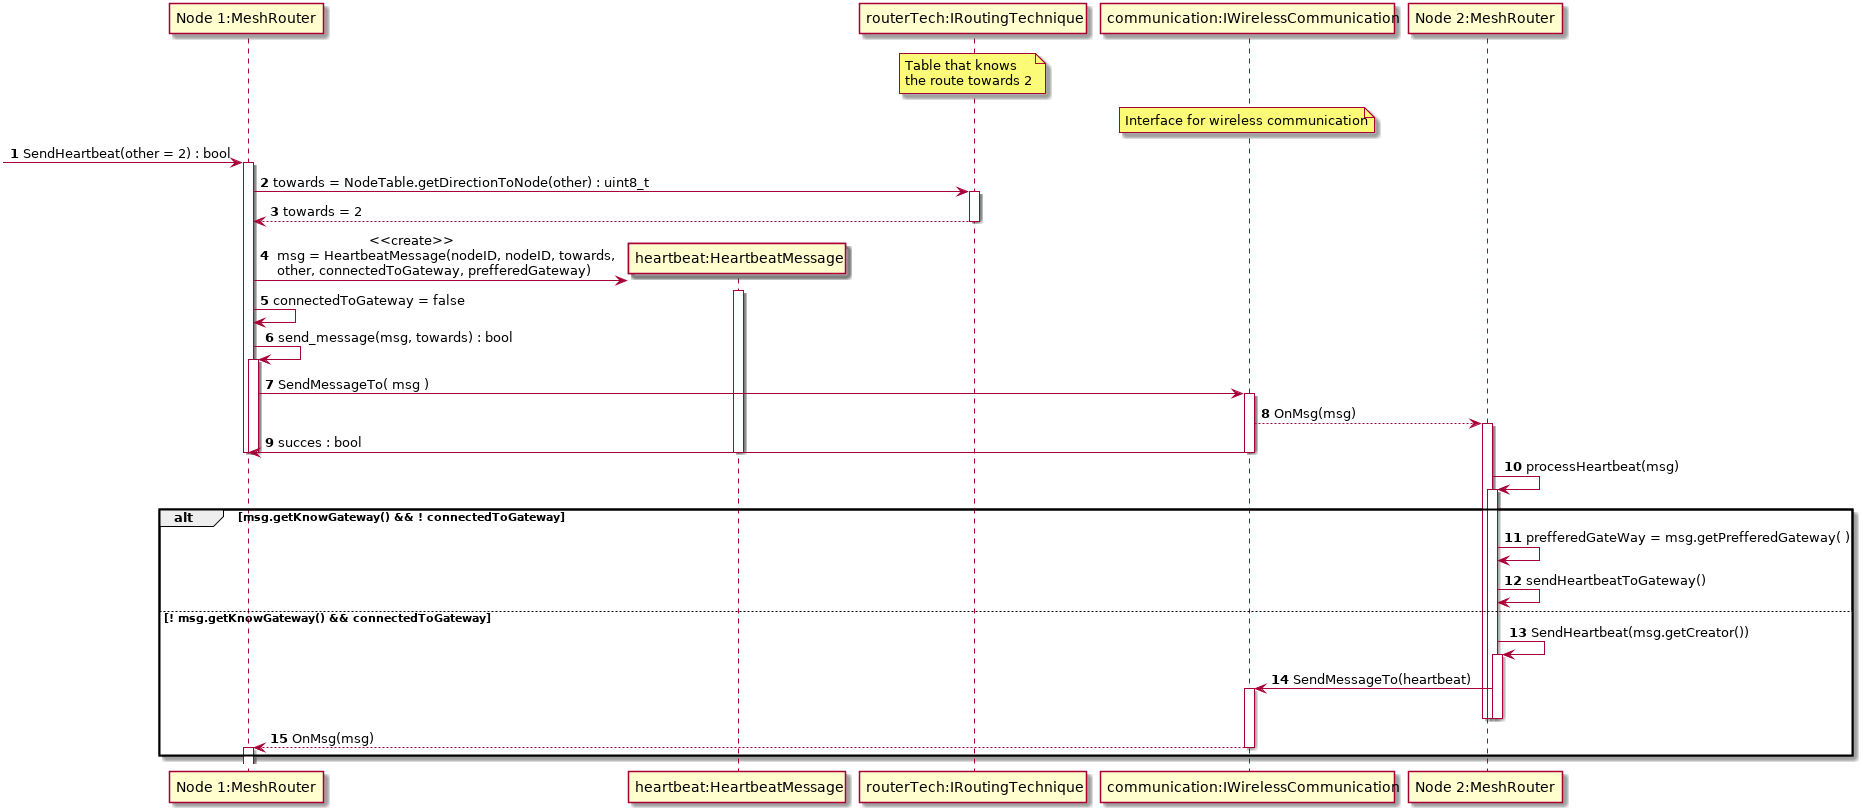
\includegraphics[width=\linewidth]{UML/out/Communication/Sequence/RouterHeartbeatRouter/RouterHeartbeatRouter.png}\end{center}
	\caption{Sequence diagram van een heartbeat bericht van een gateway naar een router via een andere router.}
	\label{fig:communication:sequence:sequence:router->router}
\end{figure}



\subsection{Activity and State Diagrams}
\label{DetailedDesign:Communicatie:Activity}
\subsection{Design decisions made for the sub-system}

\section{Design Sub-Systeem gazebo}
\label{DetailedDesign:MeshNetwerk}
\subsection{Component Diagram}
\label{DetailedDesign:MeshNetwerk:ComponentDiagram}
\begin{figure}[H]
	\begin{center}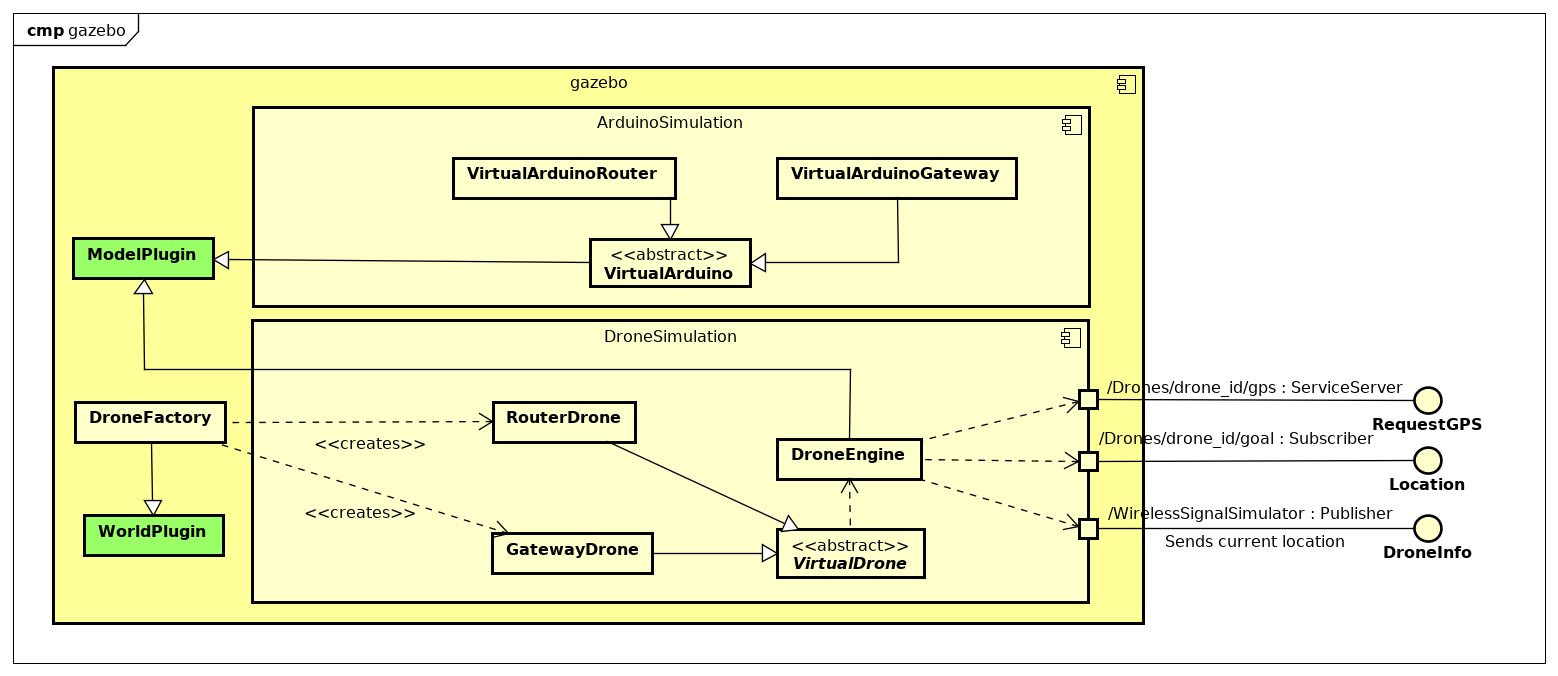
\includegraphics[width=\linewidth]{Afbeeldingen/gazeboComponentDiagram.png}\end{center}
	\caption{component diagram gazebo}
	\label{fig:component:gazebo}
\end{figure}
\subsection{Sequence Diagrams}
\label{DetailedDesign:MeshNetwerk:sequence}
\subsection{Activity and State Diagrams}
\label{DetailedDesign:MeshNetwerk:activity}
\subsection{Design decisions made for the sub-system}
\label{DetailedDesign:MeshNetwerk:decisions}

\section{Design Sub-System ros}
\label{DetailedDesign:WirelessSimulatie}
\subsection{Component Diagram}
\label{DetailedDesign:ros:ComponentDiagram}
\begin{figure}[H]
	\begin{center}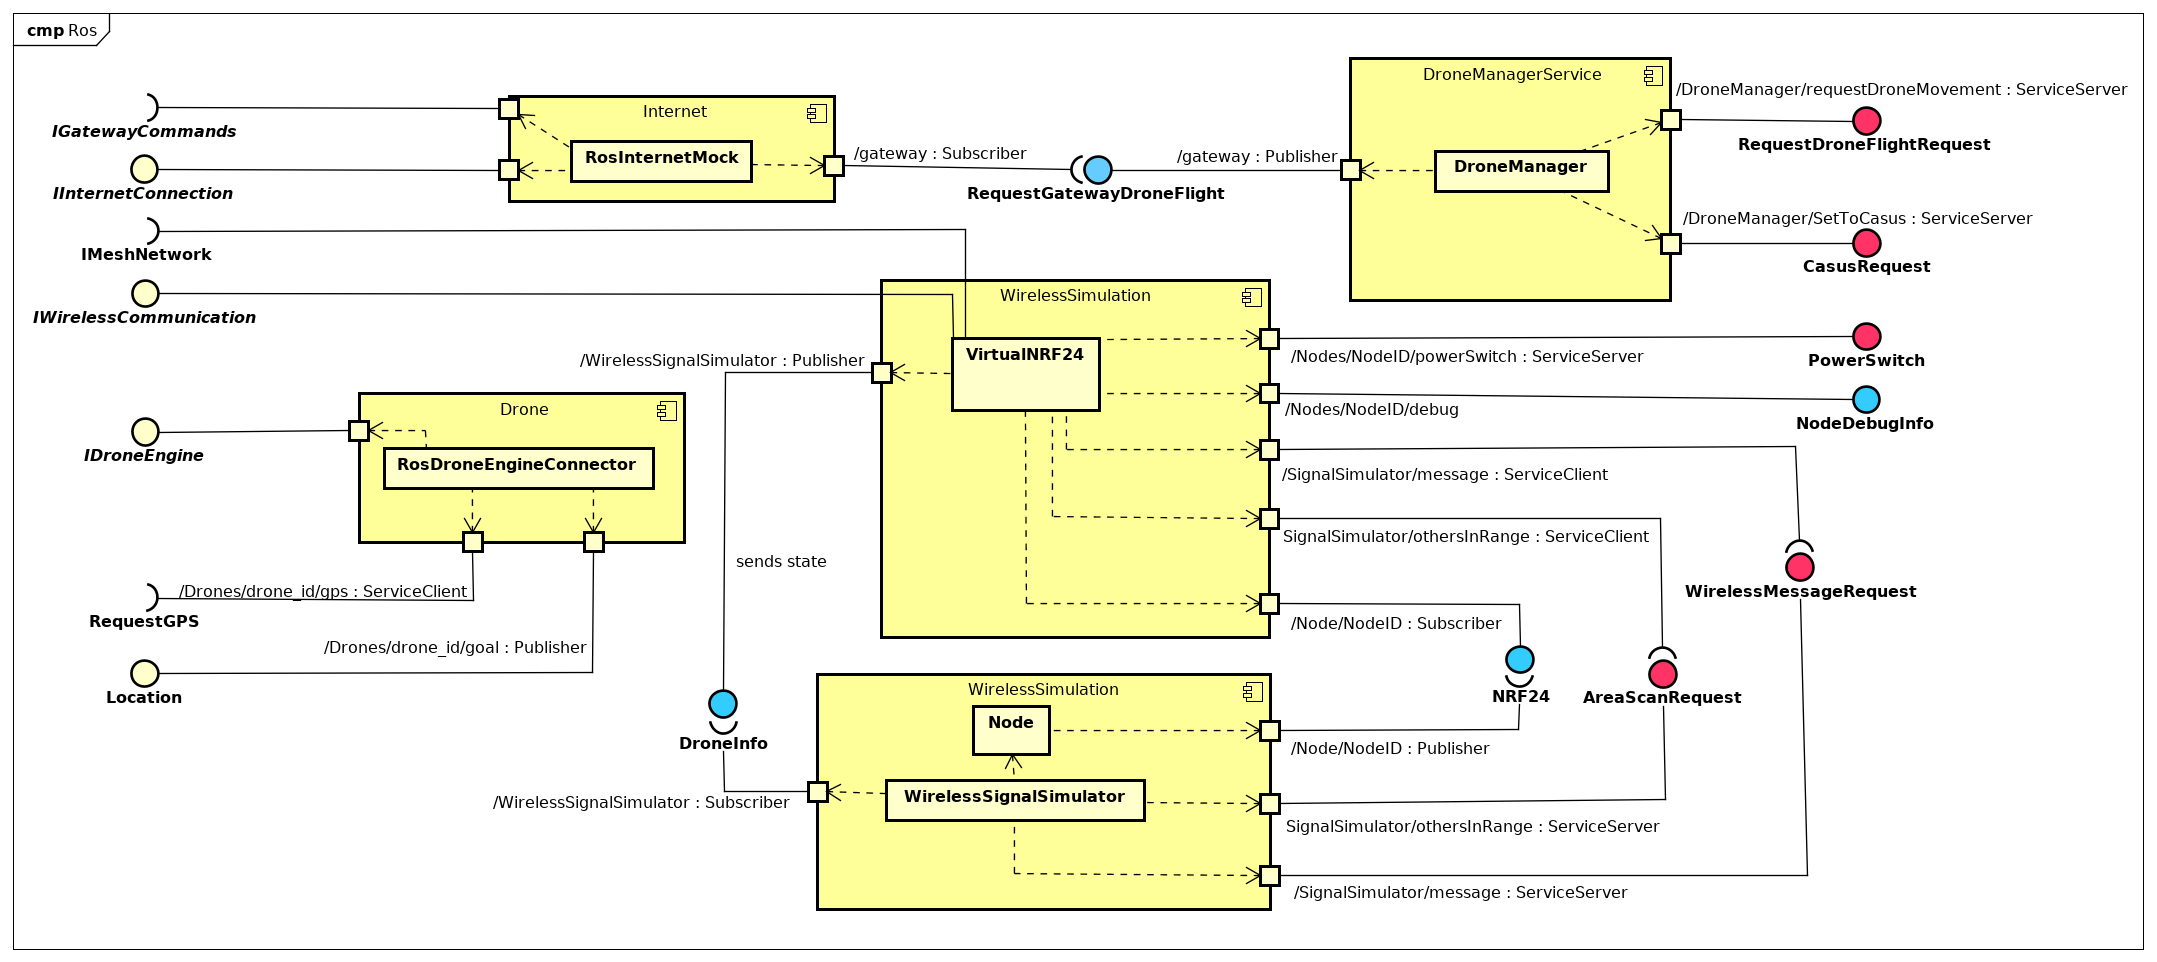
\includegraphics[width=\linewidth]{Afbeeldingen/rosComponentDiagram.png}\end{center}
	\caption{component diagram ros}
	\label{fig:component:ros}
\end{figure}
\subsection{Sequence Diagrams}
\label{DetailedDesign:WirelessSimulatie:sequence}
\subsection{Activity and State Diagrams}
\label{DetailedDesign:WirelessSimulatie:activity}
\subsection{Design decisions made for the sub-system}
\label{DetailedDesign:WirelessSimulatie:decisions}

\section{Design Sub-System NRF24}
\label{DetailedDesign:NRF24}
\subsection{Component Diagram}
\label{DetailedDesign:NRF24:ComponentDiagram}
\begin{figure}[H]
	\begin{center}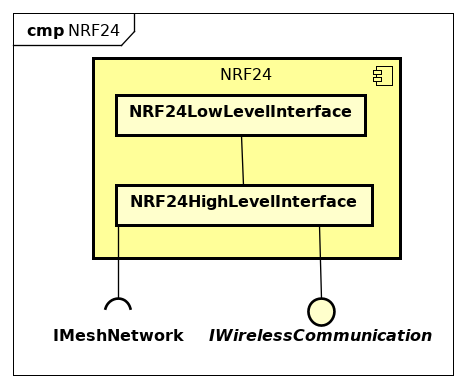
\includegraphics[width=.5\linewidth]{Afbeeldingen/NRF24ComponentDiagram.png}\end{center}
	\caption{component diagram ros}
	\label{fig:component:NRF24}
\end{figure}
\subsection{Sequence Diagrams}
\label{DetailedDesign:NRF24:sequence}
\subsection{Activity and State Diagrams}
\label{DetailedDesign:NRF24:activity}
\subsection{Design decisions made for the sub-system}
\label{DetailedDesign:NRF24:decisions}


\bibliographystyle{apacite}
\bibliography{bilbliography.bib}

\clearpage
\appendix
\chapter{Appendix 1}
\label{app:iteratieplan}





\end{document}